\documentclass[a4paper]{article}

\usepackage[english]{babel}
\usepackage[utf8]{inputenc}
\usepackage{amsmath}
\usepackage{amssymb}
\usepackage{graphicx}
\usepackage[colorinlistoftodos]{todonotes}
\usepackage{epigraph}

\setlength\parindent{0pt}

\newcommand{\ledd}{L_{\mathrm{Edd}}}
\newcommand{\medd}{\dot{M}_{\mathrm{Edd}}}
\newcommand{\xvec}{\mathbf{x}}
\newcommand{\Comment}[2]{ [{\color{red}\sc #1 :} {{\color{cyan} \it #2}}]}


\title{Mosaicing}

\author{Anna Ho}
\date{\today}

\begin{document}

\maketitle

\section{Motivation}

\subsection{Limiting angular scales}

\begin{description}
\item[Instantaneous FOV] The field of view imaged by one pointing of the interferometer. Using $D$ as the diameter of a dish:
\begin{equation}
\theta_\mathrm{PB} = (1.03 \rightarrow 1.2) \times \frac{\lambda}{D}
\end{equation}
\item[Spatial period] The largest angular scale Fourier component of the sky brightness that doesn't get resolved out is determined by the distribution of baselines. In practice, you only measure things about half that size well, and even that might be optimistic. Letting $b_\mathrm{min}$ be the minimum baseline for which you have reasonable UV coverage (i.e. it doesn't count if this is your one tiny baseline and the rest are very large),
\begin{equation}
\theta_\mathrm{LAS} = \frac{1}{2} \frac{\lambda}{b_\mathrm{min}}
\end{equation}
\end{description}

\Comment{To do}{Quantify the LAS yourself using the 'Gaussian loss' rule of thumb from the D. Wilner lecture on deconvolution}

The simplest possible scenario for an interferometer is a compact source, at a known location within your beam, much smaller than the instantaneous FOV. But in practice, your region of interest might be larger than $\theta_\mathrm{PB}$, perhaps because your sources are small and distributed over a wide area. Or, the source itself might have structure larger than $\theta_\mathrm{LAS}$. You could imagine dealing with this by using a more compact configuration (decreasing your baselines), but in practice there's a limit to how compact you can get (you can't squish the dishes together!) Often, you need to mosaic. It's very commonly required at short wavelengths, since the FOV of the interferometer decreases linearly with decreasing wavelength. 

\section{Basic description}

You tile an area of interest with pointings of your antennas that allows you to image a larger area and recover flux on angular scales larger than that implied by your shortest baseline, comparable to your primary beam. For larger scales, you might need to add single dish data.

\section{Ekers \& Rots Theorem}

This is a foundational concept of mosaicing. The idea is that because of the finite sizes of the dishes, in practice there are a range of angular scales measured by an interferometer, and UV coverage peaks at the middle of the ranges and decays off to the edges: $ \frac{\lambda}{b-D} < \theta < \frac{\lambda}{b+D} $. In other words, you don't measure a single spatial frequency, you actually measure a range of spatial frequencies. Your collection of single baseline point measurements results in a blurred, diffuse pattern, 
which is good because you get sensitivity in between the individual baseline measurements. The problem is: consider a single baseline measuring one correlation, you get one measurement. The solution is to scan the telescopes across the sky and measure the visibility many times, lets you separate out the Fourier modes, and increase the map's Fourier resolution. You're most sensitive to frequencies at the actual baseline, and because of the aperture function it falls off away from that. You're able to access information on scales larger than the shortest baseline. 

\begin{figure}
\centering
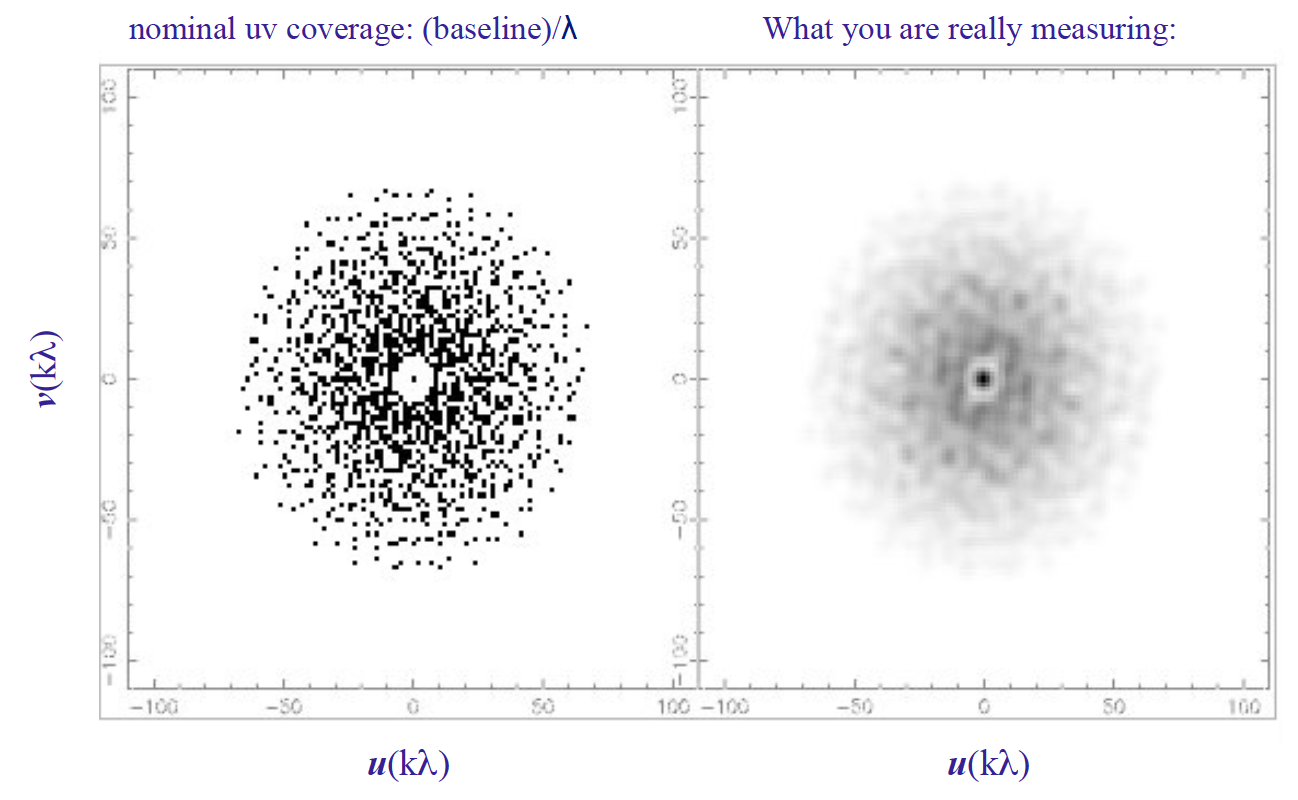
\includegraphics[width=1.0\textwidth]{EkersRots.png} 
\caption{The Ekers \& Rots Theorem says that in practice, because of finite dish size, you measure a range of spatial frequencies sensitivity that peaks at the baseline and decays out to the limits implied by the aperture.}
\label{EkersRots}
\end{figure}

In order to separate out all the Fourier modes of your measurement, you need mosaicing to measure many complex visibilities. 

\section{In Practice}

\subsection{Pointing Strategy}

There's a theoretically optimal sampling layout (Cornwell 1988) in either a rectangular grid with spacing $\frac{\lambda}{2D}$ or a hexagonal grid with spacing $\frac{2}{\sqrt{3}}\frac{\lambda}{2D}$. But if you need higher survey speed, it can make sense to space out your pointings a little more. 

\subsection{On-The-Fly Interferometry}

You scan all the antennas together across the sky, recording the data and antenna positions quickly $\rightarrow$ reduces overhead, although there's a high data rate. Scan continuously, dump correlations and all antenna positions rapidly. 

\subsection{Stitching Maps Together}

\subsubsection{Linear Combination}

You make individual pointing dirty maps, deconvolve them individually, and stitch them together at the very end of the process, assigning pointing weights from the noise and primary beam. The disadvantage is that deconvolution is only possible to the depth of an individual pointing, and it's not as effective as recovering shorter spacings. The advantage is that each pointing can be treated and calibrated separately for best results. So it can be good for high dynamic range imaging where calibration effects need to be treated with great care.
With $A(\xvec)$ as the primary response function of an antenna (the primary beam):

\begin{equation}
I(\xvec) = \frac{\Sigma_p \, A(\xvec-\xvec_p) \, I_p (\xvec)}{\Sigma_p \, A^2 (\xvec - \xvec_p)}
\end{equation}

\subsubsection{Joint Deconvolution} 
Stitch together the individual pointing dirty maps into one dirty map, deconvolve that product together (your deconvolution algorithm - clean, maximum entropy, etc - acts on a linear mosaic of dirty maps.) You form a joint dirty beam that consists of a weighted combination of the individual observations' dirty beams. Because of the nature of deconvolution algorithms, you get more large scale structure, although the approach is more sensitive to how good your model of the primary beam is. You need a spatially varying PSF. An advantage is that since you're using all $uv$ data from all points for the beam simultaneously, the combined beam provides better deconvolution in overlap regions, and ``Ekers \& Rots'' information, thus recovering more large-scale structure. However, overlapping pointings require good knowledge of the primary beam shape further out than the half power point: basically, you need a good model for the primary beam.
Introducing $W(\mathbf{x})$ as the apodization function to suppress noise amplification at the edge and $\sigma_p$ as the noise variance of an individual pointing, here's the dirty image:

\begin{equation}
I(\xvec) = W(\xvec) \frac{\Sigma_p \, A(\xvec-\xvec_p) \, I_p (\xvec) / \sigma_p^2}{\Sigma_p \, A^2 (\xvec - \xvec_p) / \sigma_p^2}
\end{equation}

You then create a joint dirty beam:

\begin{equation}
B(\xvec; \xvec_0) = W(\xvec) \frac{\Sigma_p \, A(\xvec_0-\xvec_p) \, B_p (\xvec - \xvec_0) / \sigma_p^2}{\Sigma_p \, A^2 (\xvec - \xvec_p) / \sigma_p^2}
\end{equation}

\subsubsection{Widefield Imaging}
Do the combination (of visibilities from all pointings) in the UV plane; that is, regrid the visibilities (the UV data) into a common UV plane by using a gridding kernel to phase shift each pointing to a common phase center, applying primary beam weighting (product in image space, convolution in UV domain). Use FT to create a single dirty image with a common PSF. Then deconvolve the single dirty map by the usual methods. This is what's preferred now for ALMA and a lot of VLA data; it works well with on-the-fly interferometry data (with many, many pointing centers).

\subsection{In CASA}

After calibrating as you would for a single pointing and using the clean task, use \emph{mosaic} in \emph{imagermode}, setting \emph{ftmachine='mosaic'} for wide-field imaging (this is preferred, it's faster) or \emph{ftmachine='ft'} for joint linear deconvolution. It uses the Cotton-Schwab major/minor cycle algorithm. 

\section{Issues}

\subsection{Pointings change with time}

The pointings are all taken in a time sequence. Each pointing can have different uv-coverage, atmospheric conditions, the pointing is critical because you're trying to make use of data in a place where the beam is changing quickly (instead of just in the middle, where the beam is flat). Pointing is more critical than for a non-mosaicked observation with an isolated source in the beam center. You must know your primary beam! Things are particularly tricky for extended sources because of the woes of deconvolution. 

\subsection{You're missing short \& zero spacings}

Because of the finite dish sizes, you get a hole in the middle. what does that do to your measurement? well, the effect is that you're not measuring the mean level of the sky, or even the local mean level, which results in a variable local background that can be negative.
If you imagine that your interferometer had continuous UV coverage from 0 out to some long baseline. The notch in the middle gives you these near-in negative bowls right near the central main lobe of the PSF. causes obvious and problematic effects in your maps. Looks literally like negative bowls in the middle, around the object. you can never clean all the way down, so there are residual negative side lobes. You can help with this by adding single-dish data.

\subsection{adding single-dish data}

The simplest way to add total power data to an existing interferometer map is to \textbf{feather it in}. Consider interferometer visibility measurements, binned in UV distance. Gap in the middle is the hole in the UV plane. There's generally no constraint in clean that the total flux of clean components be any particular number. So, clean will just guess a value where you don't have any data. \\

You high pass filter the interferometer data and add the single dish data. You use the single dish data where it's most effective, and don't use the interferometric data where it's least effective. \\ 

There is no cookie cutter approach to imaging extended emission with an interferometer (??) 

\end{document}